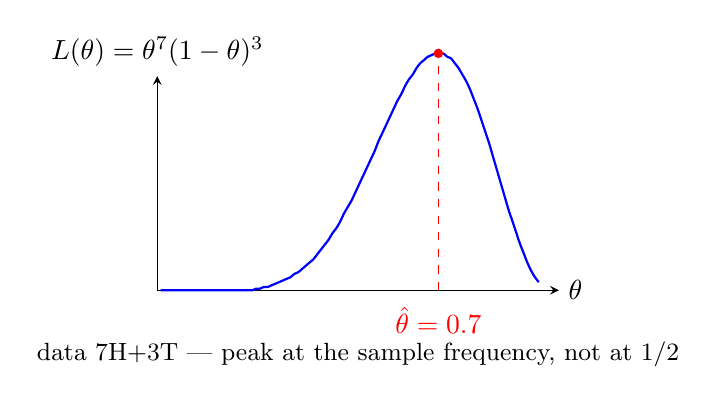
\begin{tikzpicture}[scale=0.85,>=stealth]
\draw[->] (0,0)--(6,0) node[right]{$\theta$};
\draw[->] (0,0)--(0,3.2) node[above]{$L(\theta)=\theta^{7}(1-\theta)^{3}$};
% theta^7(1-t)^3 peak at .7, max val ~.00222 scaled x800
\draw[domain=0.05:5.7,smooth,thick,blue,samples=100] plot ({\x},{1600*((\x/6)^7*(1-\x/6)^3)});
\draw[dashed,red] (4.2,0)--(4.2,{1600*(0.7^7*0.3^3)}) node[below=4pt]{};
\node[red] at (4.2,-0.45) {$\hat\theta=0.7$};
\fill[red] (4.2,{1600*(0.7^7*0.3^3)}) circle (2pt);
\node at (3,-0.95) {\small data $7$H$+3$T --- peak at the sample frequency, not at $1/2$};
\end{tikzpicture}
